\documentclass[
  man,
  floatsintext,
  longtable,
  nolmodern,
  notxfonts,
  notimes,
  colorlinks=true,linkcolor=blue,citecolor=blue,urlcolor=blue]{apa7}

\usepackage{amsmath}
\usepackage{amssymb}



\usepackage[bidi=default]{babel}
\babelprovide[main,import]{english}


% get rid of language-specific shorthands (see #6817):
\let\LanguageShortHands\languageshorthands
\def\languageshorthands#1{}

\RequirePackage{longtable}
\RequirePackage{threeparttablex}

\makeatletter
\renewcommand{\paragraph}{\@startsection{paragraph}{4}{\parindent}%
	{0\baselineskip \@plus 0.2ex \@minus 0.2ex}%
	{-.5em}%
	{\normalfont\normalsize\bfseries\typesectitle}}

\renewcommand{\subparagraph}[1]{\@startsection{subparagraph}{5}{0.5em}%
	{0\baselineskip \@plus 0.2ex \@minus 0.2ex}%
	{-\z@\relax}%
	{\normalfont\normalsize\bfseries\itshape\hspace{\parindent}{#1}\textit{\addperi}}{\relax}}
\makeatother




\usepackage{longtable, booktabs, multirow, multicol, colortbl, hhline, caption, array, float, xpatch}
\setcounter{topnumber}{2}
\setcounter{bottomnumber}{2}
\setcounter{totalnumber}{4}
\renewcommand{\topfraction}{0.85}
\renewcommand{\bottomfraction}{0.85}
\renewcommand{\textfraction}{0.15}
\renewcommand{\floatpagefraction}{0.7}

\usepackage{tcolorbox}
\tcbuselibrary{listings,theorems, breakable, skins}
\usepackage{fontawesome5}

\definecolor{quarto-callout-color}{HTML}{909090}
\definecolor{quarto-callout-note-color}{HTML}{0758E5}
\definecolor{quarto-callout-important-color}{HTML}{CC1914}
\definecolor{quarto-callout-warning-color}{HTML}{EB9113}
\definecolor{quarto-callout-tip-color}{HTML}{00A047}
\definecolor{quarto-callout-caution-color}{HTML}{FC5300}
\definecolor{quarto-callout-color-frame}{HTML}{ACACAC}
\definecolor{quarto-callout-note-color-frame}{HTML}{4582EC}
\definecolor{quarto-callout-important-color-frame}{HTML}{D9534F}
\definecolor{quarto-callout-warning-color-frame}{HTML}{F0AD4E}
\definecolor{quarto-callout-tip-color-frame}{HTML}{02B875}
\definecolor{quarto-callout-caution-color-frame}{HTML}{FD7E14}

%\newlength\Oldarrayrulewidth
%\newlength\Oldtabcolsep


\usepackage{hyperref}




\providecommand{\tightlist}{%
  \setlength{\itemsep}{0pt}\setlength{\parskip}{0pt}}
\usepackage{longtable,booktabs,array}
\usepackage{calc} % for calculating minipage widths
% Correct order of tables after \paragraph or \subparagraph
\usepackage{etoolbox}
\makeatletter
\patchcmd\longtable{\par}{\if@noskipsec\mbox{}\fi\par}{}{}
\makeatother
% Allow footnotes in longtable head/foot
\IfFileExists{footnotehyper.sty}{\usepackage{footnotehyper}}{\usepackage{footnote}}
\makesavenoteenv{longtable}

\usepackage{graphicx}
\makeatletter
\newsavebox\pandoc@box
\newcommand*\pandocbounded[1]{% scales image to fit in text height/width
  \sbox\pandoc@box{#1}%
  \Gscale@div\@tempa{\textheight}{\dimexpr\ht\pandoc@box+\dp\pandoc@box\relax}%
  \Gscale@div\@tempb{\linewidth}{\wd\pandoc@box}%
  \ifdim\@tempb\p@<\@tempa\p@\let\@tempa\@tempb\fi% select the smaller of both
  \ifdim\@tempa\p@<\p@\scalebox{\@tempa}{\usebox\pandoc@box}%
  \else\usebox{\pandoc@box}%
  \fi%
}
% Set default figure placement to htbp
\def\fps@figure{htbp}
\makeatother


% definitions for citeproc citations
\NewDocumentCommand\citeproctext{}{}
\NewDocumentCommand\citeproc{mm}{%
  \begingroup\def\citeproctext{#2}\cite{#1}\endgroup}
\makeatletter
 % allow citations to break across lines
 \let\@cite@ofmt\@firstofone
 % avoid brackets around text for \cite:
 \def\@biblabel#1{}
 \def\@cite#1#2{{#1\if@tempswa , #2\fi}}
\makeatother
\newlength{\cslhangindent}
\setlength{\cslhangindent}{1.5em}
\newlength{\csllabelwidth}
\setlength{\csllabelwidth}{3em}
\newenvironment{CSLReferences}[2] % #1 hanging-indent, #2 entry-spacing
 {\begin{list}{}{%
  \setlength{\itemindent}{0pt}
  \setlength{\leftmargin}{0pt}
  \setlength{\parsep}{0pt}
  % turn on hanging indent if param 1 is 1
  \ifodd #1
   \setlength{\leftmargin}{\cslhangindent}
   \setlength{\itemindent}{-1\cslhangindent}
  \fi
  % set entry spacing
  \setlength{\itemsep}{#2\baselineskip}}}
 {\end{list}}
\usepackage{calc}
\newcommand{\CSLBlock}[1]{\hfill\break\parbox[t]{\linewidth}{\strut\ignorespaces#1\strut}}
\newcommand{\CSLLeftMargin}[1]{\parbox[t]{\csllabelwidth}{\strut#1\strut}}
\newcommand{\CSLRightInline}[1]{\parbox[t]{\linewidth - \csllabelwidth}{\strut#1\strut}}
\newcommand{\CSLIndent}[1]{\hspace{\cslhangindent}#1}





\usepackage{newtx}

\defaultfontfeatures{Scale=MatchLowercase}
\defaultfontfeatures[\rmfamily]{Ligatures=TeX,Scale=1}





\title{Education Funding Inequality and Academic Performance Disparity
between Migrant and Local Students in China}


\shorttitle{D2MR Final Project}


\usepackage{etoolbox}






\author{Jiayi Zou}



\affiliation{
{MA Program in the Social Sciences, University of Chicago}}




\leftheader{Zou}



\abstract{This document is a template demonstrating the apaquarto
format. It includes examples of how to create figures and tables, as
well as how to reference them in the text. The document is written in
Quarto, a system for creating documents with R Markdown. The apaquarto
extension provides a template for creating APA7-formatted manuscripts. }

\keywords{education inequality, internal migration, education
funding, fiscal decentralization}

\authornote{ 

\par{  This project is the final assignment for Data to Manuscript in R
(D2MR) instructed by Dr.~Natalie Dowling. It also serves as an interim
result of Jiayi Zou's MA thesis project.   The author is grateful
Dr.~Dowling for supporting this project and offering guidance throughout
the quarter.  }
\par{Correspondence concerning this article should be addressed to Jiayi
Zou, MA Program in the Social Sciences, University of Chicago, 1155 E
60th St., Chicago, IL 60637, USA, Email: jiayizou@uchicago.edu}
}

\makeatletter
\let\endoldlt\endlongtable
\def\endlongtable{
\hline
\endoldlt
}
\makeatother

\urlstyle{same}



\makeatletter
\@ifpackageloaded{caption}{}{\usepackage{caption}}
\AtBeginDocument{%
\ifdefined\contentsname
  \renewcommand*\contentsname{Table of contents}
\else
  \newcommand\contentsname{Table of contents}
\fi
\ifdefined\listfigurename
  \renewcommand*\listfigurename{List of Figures}
\else
  \newcommand\listfigurename{List of Figures}
\fi
\ifdefined\listtablename
  \renewcommand*\listtablename{List of Tables}
\else
  \newcommand\listtablename{List of Tables}
\fi
\ifdefined\figurename
  \renewcommand*\figurename{Figure}
\else
  \newcommand\figurename{Figure}
\fi
\ifdefined\tablename
  \renewcommand*\tablename{Table}
\else
  \newcommand\tablename{Table}
\fi
}
\@ifpackageloaded{float}{}{\usepackage{float}}
\floatstyle{ruled}
\@ifundefined{c@chapter}{\newfloat{codelisting}{h}{lop}}{\newfloat{codelisting}{h}{lop}[chapter]}
\floatname{codelisting}{Listing}
\newcommand*\listoflistings{\listof{codelisting}{List of Listings}}
\makeatother
\makeatletter
\makeatother
\makeatletter
\@ifpackageloaded{caption}{}{\usepackage{caption}}
\@ifpackageloaded{subcaption}{}{\usepackage{subcaption}}
\makeatother

% From https://tex.stackexchange.com/a/645996/211326
%%% apa7 doesn't want to add appendix section titles in the toc
%%% let's make it do it
\makeatletter
\xpatchcmd{\appendix}
  {\par}
  {\addcontentsline{toc}{section}{\@currentlabelname}\par}
  {}{}
\makeatother

%% Disable longtable counter
%% https://tex.stackexchange.com/a/248395/211326

\usepackage{etoolbox}

\makeatletter
\patchcmd{\LT@caption}
  {\bgroup}
  {\bgroup\global\LTpatch@captiontrue}
  {}{}
\patchcmd{\longtable}
  {\par}
  {\par\global\LTpatch@captionfalse}
  {}{}
\apptocmd{\endlongtable}
  {\ifLTpatch@caption\else\addtocounter{table}{-1}\fi}
  {}{}
\newif\ifLTpatch@caption
\makeatother

\begin{document}

\maketitle


\setcounter{secnumdepth}{-\maxdimen} % remove section numbering

\setlength\LTleft{0pt}


\section{Introduction}\label{introduction}

Internal migration in China has accelerated along with urbanization
since the implementation of Reform and Opening Up policy in the early
1980s. Statistics from the 7th National Census in 2020 show that over 70
million children in China have migration status, which means one fourth
of Chinese child population move interprovincially or intraprovincially
with their parents \footnote{See in
  \href{https://www.163.com/dy/article/JHFCU34705560ZWH.html}{Promoting
  reunion and avoiding separation - China's migrant children development
  report 2024}.}. Education and sociology research focusing on internal
migrant students found that these children have a relatively lower
school achievement compared to local students without migrant status,
and suffer from academic and financial difficulties, as well as
alienation in public education system
(\citeproc{ref-chenAccessPublicSchools2013}{Chen \& Feng, 2013};
\citeproc{ref-huangMythMigrantsProblems2017a}{Huang, 2017}).

Previous studies offered policy explanations for migrant students'
underachievement. Li (\citeproc{ref-liDataAnalysisCurrent2018}{2018})
indicated that central governments have less educational funding
distributed to provinces containing more migrant population due to
fiscal decentralization. On the other hand, the \emph{Hukou} policy
\footnote{The \emph{Hukou} Policy is a population management policy that
  restraints non-local residents from/uplifts the threshold of enjoying
  the same social, medical, and educational public services as local
  households do.} has a history of limiting policy supports for internal
migrants including subsidies, fee standards, and other financial
accesses, which contributes migrant students' underperformance in school
(\citeproc{ref-luVillagersCityResilience2023}{Lu, 2023}).

However, both perspectives have failed to identify an integrated
framework: if we can discover the impact of differentiated financial
supports and per student funding appropriated to two groups of students,
then it is plausible to assume that fiscal decentralization is producing
local-migrant educational inequity through the lens of \emph{Hukou}
status.

In this study, I seek to understand \textbf{how governments'
differentiated provision of education fundings affects the academic
performance disparity between migrant students and local students in
China} . My hypothesis is \textbf{when the government provides migrant
students with limited fundings, and less-supportive charging standards
and subsidy policies, the academic performance gap between the two
groups of students is likely to widen}.

Beyond measuring educational disparities created by the complexity of
fiscal decentralization and population management system, this research
has practical significance for addressing the ongoing migrant problems
in China's urban governance and the institution of compulsory education
(\citeproc{ref-nationalbureauofstatisticsofchinaetal_2023_what}{National
Bureau of Statistics of China et al., 2023}). Last but not least, this
study can also offer indications for how educational finance and
policies provided by government interacts with structural inequality in
other social contexts (e.g., areas with higher poverty level or racial
disparities, see in studies by Baird
(\citeproc{ref-baird_2008_federal}{2008}) and Hyman
(\citeproc{ref-hyman_2017_does}{2017})).

\section{Literature Review}\label{literature-review}

In this study, we define \emph{provision of education fundings} as a
combination of three elements: (1) the amount of funding, including
per-student funding, subsidies, and charging standards; (2) the
proportion of funding, which is seperated into central/provincial and
county/district level; and (3) the indicator of differentiation, which
is whether migrant students enjoy the equal educational financial
resources as locally-registered students in terms of funding, subsidies,
and charging standards. Inspired by Knoeppel and Della Sala
(\citeproc{ref-knoeppelEducationFundingStudent2015}{2015}), we consider
that education funding, influenced by fiscal decentralization and
\emph{Hukou} system, affects migrant and local students in the same
schools through context for schooling, which results in unequal academic
performances between two student groups.

\subsection{Education Funding and Academic
Achievement}\label{education-funding-and-academic-achievement}

Scholarship in education funding suggests that students of color have
been continuously underfunded by federal and state, and the discrepancy
between their and higher-SES/white counterparts' academic performance
persists (\citeproc{ref-darling-hammond_2004_color}{Darling-Hammond,
2004}; \citeproc{ref-gaddislauen_2014_school}{Gaddis \& Lauen, 2014};
\citeproc{ref-lafortuneetal_2018_school}{Lafortune et al., 2018};
\citeproc{ref-ryan_1999_schools}{Ryan, 1999}). In China, researchers
found similar patterns and disparities among migrant students and
local-\emph{Hukou} students. Evidence from China Education Paney survey
indicates that local students outperform migrant students at higher
quantile point, and increasing total education expenditure is likely
shrink the academic achievement gap
(\citeproc{ref-fangStudyOutcomeEquity2024}{Fang \& Zhang, 2024}).
However, the association between other aspects of education expenditure
(e.g.~per student funding, central and local government appropriation
ratio) and local-migrant academic outcome equity requires further
exploration, as most studies center on how funding expands spatial
education inequity rather than disparities between different
\emph{Hukou} statuses in cities
(\citeproc{ref-weiAnalysisReportUrbanrural2022}{Wei et al., 2022}).

\subsection{Fiscal Decentralization and Descriminatory Policies against
Internal
Migrants}\label{fiscal-decentralization-and-descriminatory-policies-against-internal-migrants}

Beyond education finance disparities, education policies also differ for
migrant and local students in many provinces, which means students
without local registration (\emph{hukou}) may have no government
subsidies or face different charging standards. Researchers refer this
phenomenon as deflecting internal migrants' demands and using education
to control urban population influx
(\citeproc{ref-chanPhantomServicesDeflecting2019}{Chan \& O'Brien,
2019}; \citeproc{ref-friedmanBiopoliticsUrbanizationChina2018}{Friedman,
2018}). The disadvantage encountered by migran students varies in
different city scenarios: if local education policy background is more
\emph{Hukou}-based discriminatory, then migrant students are more likely
to receive lower school performance than local students
(\citeproc{ref-maMigrantStatusSchool2020}{Ma, 2020}). Deflecting
education resources away from the underprivileged students occurs in
U.S. schools to avoid losing fundings under school accountability, as
the minority subgroups have a higher possibility to fall short of the
average academic target
(\citeproc{ref-hanushekraymond_2005_does}{Hanushek \& Raymond, 2005};
\citeproc{ref-oday_2009_complexity}{O'Day, 2009}). Similarly, turning
down education fundings for migrant students is also a strategy for
Chinese local governments to decrease overall financial stress due to
fiscal decentralization
(\citeproc{ref-jinRegionalDecentralizationFiscal2005a}{Jin et al.,
2005}; \citeproc{ref-longFiscalDecentralisationKnowledge2017}{Long et
al., 2017}).

As migrant students represent social minorities with limited or without
\emph{Hukou}-related rights in urban spaces, exploring their education
achievements influenced by government funding and financial supports can
demonstrate the dynamic and diverse efficiency of providing public
services, offering empirical evidence for the development of
decentralization theory
(\citeproc{ref-oatesSecondGenerationTheoryFiscal2005}{Oates, 2005},
\citeproc{ref-oates_2008_evolution}{2008}).

\section{Data and Methods}\label{data-and-methods}

\subsection{Data}\label{data}

In this project, we use the follow-up (2014-2015) dataset from the China
Education Panel Survey
\href{http://ceps.ruc.edu.cn/English/Home.htm}{CEPS}. CEPS is conducted
by National Survey Research Center at Renmin University of China and it
is the most used dataset in studies of Chinese internal migrant
students. Data includes 1769 migrant students and 7960 non-migrant
students who have were at 9th Grade as in the final year of Junior High.
We will merge datasets based on student, class, and school id, and
remove values without valid information of hukou status.

\subsection{Measures}\label{measures}

The dependent variable in our study is the academic performance, which
is measured by three indexes: score (percentage) of Chinese,
Mathematics, and English exams. In
Figure~\ref{fig-box-academic-performance}, a primary investigation into
the follow-up dataset suggests that the medium and average of all three
test scores for migrant students are all less than the equivalents for
non-migrant students. Additionally, migrant students performances in
Chinese and English exams are more concentrated than local students, but
possibly due to different sample size. More outliers in Chinese exam
scores appeared in migrant student group than their local counterparts,
suggesting migrant students might experience greater difficulty in
achieveing in Chinese exams.

\begin{figure}[H]

\caption{\label{fig-box-academic-performance}Comparison of the
Distribution of Chinese, Mathematics, and English Exam Scores between
Local Students and Migrant Students}

\centering{

\pandocbounded{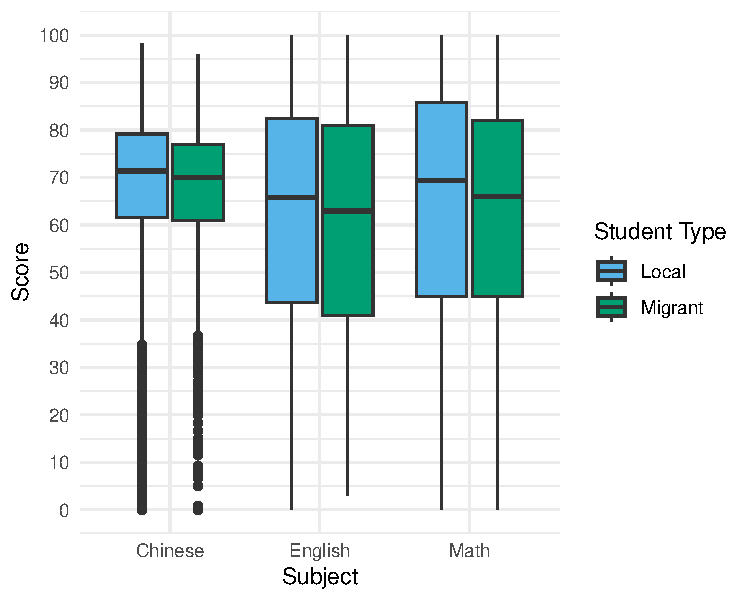
\includegraphics[keepaspectratio]{migrant-student-education_files/figure-pdf/fig-box-academic-performance-1.pdf}}

}

\end{figure}%

As for the independent variable, we take three aspects into account: the
amount of per-student funding and subsidies; the proportion of funding
sources, which is seperated into central/provincial level and
county/district level; and whether migrant students enjoy the equal
funding, subsidies, and charging standards as locally-registered
students do.

\subsection{Methods}\label{methods}

\section{Analysis Results}\label{analysis-results}

\section{Conclusion}\label{conclusion}

\clearpage

\section{References}\label{references}

\phantomsection\label{refs}
\begin{CSLReferences}{1}{0}
\bibitem[\citeproctext]{ref-baird_2008_federal}
Baird, K. E. (2008). Federal {Direct Expenditures} and {School Funding
Disparities}, 1990-2000. \emph{Journal of Education Finance},
\emph{33}(3), 297--310. \url{https://www.jstor.org/stable/40704331}

\bibitem[\citeproctext]{ref-chanPhantomServicesDeflecting2019}
Chan, A. T., \& O'Brien, K. J. (2019). Phantom {Services}: {Deflecting
Migrant Workers} in {China}. \emph{The China Journal}, \emph{81},
103--122. \url{https://doi.org/10.1086/699215}

\bibitem[\citeproctext]{ref-chenAccessPublicSchools2013}
Chen, Y., \& Feng, S. (2013). Access to public schools and the education
of migrant children in {China}. \emph{China Economic Review}, \emph{26},
75--88. \url{https://doi.org/10.1016/j.chieco.2013.04.007}

\bibitem[\citeproctext]{ref-darling-hammond_2004_color}
Darling-Hammond, L. (2004). {THE COLOR LINE IN AMERICAN EDUCATION}:
{Race}, {Resources}, and {Student Achievement}. \emph{Du Bois Review:
Social Science Research on Race}, \emph{1}(2), 213--246.
\url{https://doi.org/10.1017/S1742058X0404202X}

\bibitem[\citeproctext]{ref-fangStudyOutcomeEquity2024}
Fang, C., \& Zhang, Y. (2024). {A Study on the Outcome Equity of
Compulsory Education for Local and Migrant Children and the Financial
Input and Expenditure of Family Education}. \emph{Basic Education
Review}, \emph{368}(08), 3--17.
\url{https://doi.org/10.3969/j.issn.1672-1128.2024.08.001}

\bibitem[\citeproctext]{ref-friedmanBiopoliticsUrbanizationChina2018}
Friedman, E. (2018). The {Biopolitics} of {Urbanization} in {China}:
{Managing Migration} and {Access} to {Education}. In
\emph{Developmentalist {Cities}? {Interrogating Urban Developmentalism}
in {East Asia}} (pp. 68--90). Brill.
\url{https://doi.org/10.1163/9789004383609_005}

\bibitem[\citeproctext]{ref-gaddislauen_2014_school}
Gaddis, S. M., \& Lauen, D. L. (2014). School accountability and the
black--white test score gap. \emph{Social Science Research}, \emph{44},
15--31. \url{https://doi.org/10.1016/j.ssresearch.2013.10.008}

\bibitem[\citeproctext]{ref-hanushekraymond_2005_does}
Hanushek, E. A., \& Raymond, M. E. (2005). Does school accountability
lead to improved student performance? \emph{Journal of Policy Analysis
and Management}, \emph{24}(2), 297--327.
\url{https://doi.org/10.1002/pam.20091}

\bibitem[\citeproctext]{ref-huangMythMigrantsProblems2017a}
Huang, E. (2017). The myth of 'migrants as problems': {Public} school in
neoliberal times and the construction and contestation of 'migrant'
identity. \emph{Journal of Language, Identity, and Education},
\emph{16}(6), 381--394.
\url{https://doi.org/10.1080/15348458.2017.1381022}

\bibitem[\citeproctext]{ref-hyman_2017_does}
Hyman, J. (2017). Does {Money Matter} in the {Long Run}? {Effects} of
{School Spending} on {Educational Attainment}. \emph{American Economic
Journal: Economic Policy}, \emph{9}(4), 256--280.
\url{https://www.jstor.org/stable/26598353}

\bibitem[\citeproctext]{ref-jinRegionalDecentralizationFiscal2005a}
Jin, H., Qian, Y., \& Weingast, B. R. (2005). Regional decentralization
and fiscal incentives: {Federalism}, {Chinese} style. \emph{Journal of
Public Economics}, \emph{89}(9-10), 1719--1742.
\url{https://doi.org/10.1016/j.jpubeco.2004.11.008}

\bibitem[\citeproctext]{ref-knoeppelEducationFundingStudent2015}
Knoeppel, R. C., \& Della Sala, M. R. (2015). Education {Funding} and
{Student Outcomes}: {A Conceptual Framework} for {Measurement} of the
{Alignment} of {State Education Finance} and {Academic Accountability
Policies}. \emph{Educational Considerations}, \emph{42}(2).
\url{https://doi.org/10.4148/0146-9282.1050}

\bibitem[\citeproctext]{ref-lafortuneetal_2018_school}
Lafortune, J., Rothstein, J., \& Schanzenbach, D. W. (2018). School
{Finance Reform} and the {Distribution} of {Student Achievement}.
\emph{American Economic Journal: Applied Economics}, \emph{10}(2),
1--26. \url{https://www.jstor.org/stable/26528381}

\bibitem[\citeproctext]{ref-liDataAnalysisCurrent2018}
Li, N. (2018). \emph{{Data analysis: Current situation, problems and
countermeasures of the financial system of compulsory education for
migrant children}}.
https://www.thepaper.cn/newsDetail\_forward\_2673802.

\bibitem[\citeproctext]{ref-longFiscalDecentralisationKnowledge2017}
Long, Y., Nyland, C., \& Smyth, R. (2017). Fiscal {Decentralisation},
the {Knowledge Economy} and {School Teachers}' {Wages} in {Urban China}.
\emph{Journal of Development Studies}, \emph{53}(10), 1731--1747.

\bibitem[\citeproctext]{ref-luVillagersCityResilience2023}
Lu, S. (2023). '{Villagers} in the {City}': {Resilience} in migrant
youth amidst urbanisation. \emph{British Journal of Social Work},
\emph{53}(1), 236--257. \url{https://doi.org/10.1093/bjsw/bcac122}

\bibitem[\citeproctext]{ref-maMigrantStatusSchool2020}
Ma, G. (2020). Migrant status, school segregation, and students'
academic achievement in urban {China}. \emph{Chinese Sociological
Review}, \emph{52}(3), 319--336.

\bibitem[\citeproctext]{ref-nationalbureauofstatisticsofchinaetal_2023_what}
National Bureau of Statistics of China, UNICEF China, \& UNFPA China.
(2023). \emph{What the 2020 {Census Can Tell Us About Children} in
{China}: {Facts} and {Figures}}.
https://www.unicef.cn/en/reports/population-status-children-china-2020-census.

\bibitem[\citeproctext]{ref-oday_2009_complexity}
O'Day, J. (2009). Complexity, {Accountability}, and {School
Improvement}. \emph{Harvard Educational Review}, \emph{72}(3), 293--329.
\url{https://doi.org/10.17763/haer.72.3.021q742t8182h238}

\bibitem[\citeproctext]{ref-oatesSecondGenerationTheoryFiscal2005}
Oates, W. E. (2005). Toward a {Second-Generation Theory} of {Fiscal
Federalism}. \emph{International Tax \& Public Finance}, \emph{12}(4),
349--373. \url{https://doi.org/10.1007/s10797-005-1619-9}

\bibitem[\citeproctext]{ref-oates_2008_evolution}
Oates, W. E. (2008). On {The Evolution} of {Fiscal Federalism}: {Theory}
and {Institutions}. \emph{National Tax Journal}, \emph{61}(2), 313--334.
\url{https://www.jstor.org/stable/41790447}

\bibitem[\citeproctext]{ref-ryan_1999_schools}
Ryan, J. E. (1999). Schools, {Race}, and {Money}. \emph{The Yale Law
Journal}, \emph{109}(2), 249--316. \url{https://doi.org/10.2307/797490}

\bibitem[\citeproctext]{ref-weiAnalysisReportUrbanrural2022}
Wei, Y., Zhu, L., \& Ji, C. (2022). \emph{Analysis report on the
urban-rural gap of the per-student expenditure level of compulsory
education in {China}}. Institute of Chinese Educational Finance Science,
Peking University.

\end{CSLReferences}






\end{document}
